
\documentclass[afourpaper]{latex-classes/handout}

\title{Fraktale Bildcodierung}
\author{Jens Ochsenmeier}
\date{}

\newcommand{\marginrule}{\makebox[\linewidth]{\rule{\linewidth}{0.4pt}}}

\mathcode`\*="8000
{\catcode`\*\active\gdef*{\cdot}}

\definecolor{kitGreen}{HTML}{32A189}
\renewcommand{\emph}[1]{\textcolor{kitGreen}{#1}}

\begin{document}

\maketitle

\section{Die Menge aller echten Bilder}

\begin{marginfigure}[8em]
  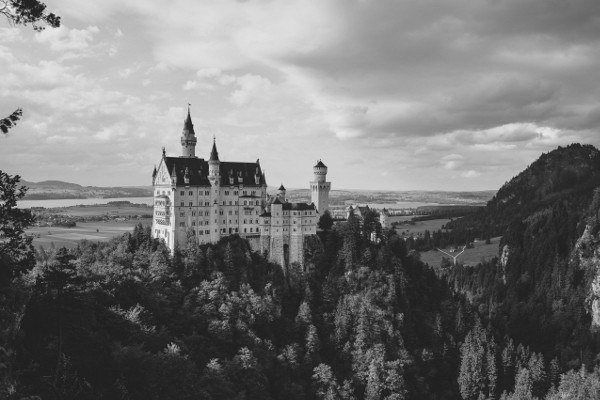
\includegraphics[width=\linewidth]{neuschwanstein-sw}
  \footnotesize{Ein ``echtes'' Bild. Offensichtlich erfüllt es die erste Eigenschaft, da es gedruckt ist und somit einen endlichen Träger (dieses Blatt) besitzt. \\ In diesem Vortrag werden wir uns auf Bilder mit Graustufen beschränken. Die erklärten Prinzipien funktionieren uneingeschränkt für farbige Bilder, sind aber etwas komplexer zu notieren.}
  \marginrule{}
\end{marginfigure}

Ein \textbf{echtes Bild} ist nicht direkt mathematisch greifbar --- es ist etwas, dass man irgendwo sehen oder sich zumindest zu sehen vorstellen könnte. Wir nennen
\begin{itemize}
  \item \( \mathcal{R} \) die Menge der echten Bilder und
  \item \( \mathcal{I} \in \mathcal{R} \) ein echtes Bild.
\end{itemize}
Ein solches \( \mathcal{I} \) muss folgende Eigenschaften erfüllen:

\begin{marginfigure}
  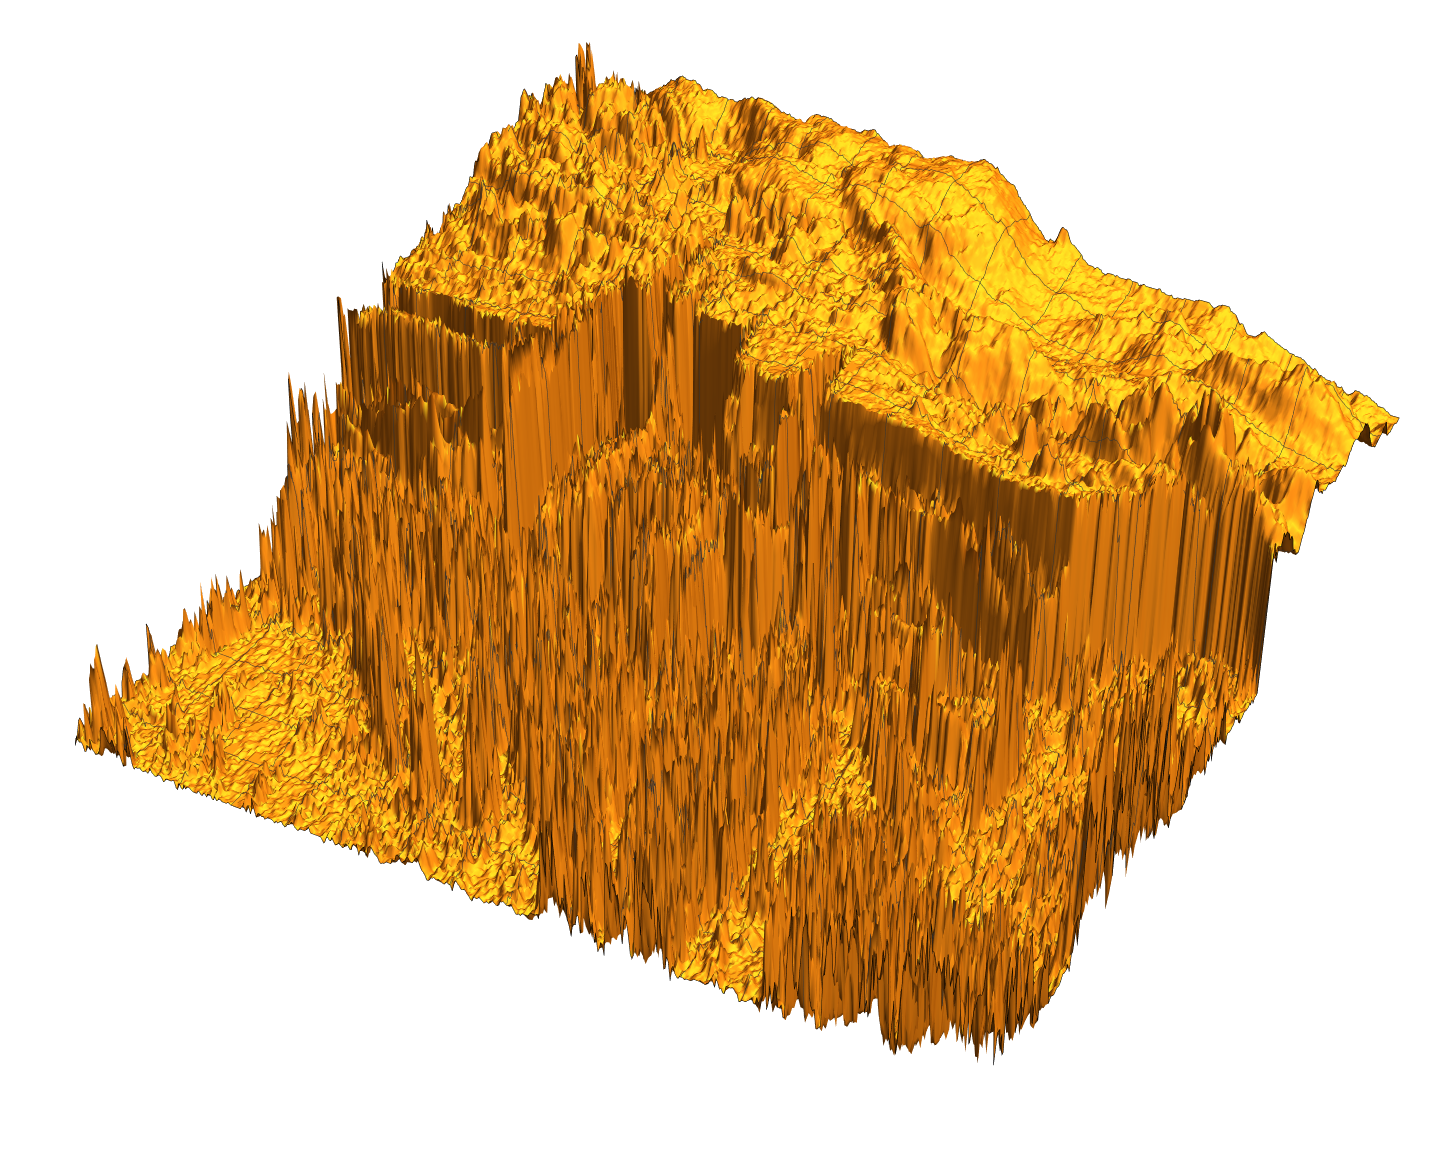
\includegraphics[width=\linewidth]{neuschwanstein-chromatic}
  \footnotesize{Plot der chromatischen Funktion \( c \) für das gegebene Bild. Man erkennt, dass die Funktionswerte in der oberen Hälfte des Bildes größer sind; dort ist das Bild heller.}
  \marginrule{}
\end{marginfigure}

\begin{enumerate}
  \item Es besitzt einen \textbf{Träger} \( \largesquare = [a,b] \times [c,d] \subset \R^2 \) und die \textbf{Maße} \( (b-a) \) und \( (d-c) \).

  \item Es besitzt gewisse \textbf{chromatische Werte} \( c_i: \largesquare \to \R \), welche jedem Punkt des Bildes einen reellwertigen Wert zuordnet.

  \item Einem Bild \( \mathcal{I} \in \mathcal{R} \) ist \ital{keine} Auflösung zugeordnet --- verschiedene Auflösungen beschreiben dasselbe Bild. Rasterung ist nicht Teil dieses Vortrags.

  \item \( \mathcal{R} \) ist unter Zuschneiden von Bildern abgeschlossen.
  \item \( \mathcal{R} \) ist unter invertierbaren affinen Transformationen abgeschlossen.
\end{enumerate}

\section{Collage-Theorem}

\begin{marginfigure}
  \textbf{Zutaten für das Collage-Theorem}:
  \begin{itemize}
    \item vollständiger metrischer Raum \( (X,d) \)
    \item \( L \in \mathcal{H}(X) \)
    \item \( \epsilon \geq 0 \)
    \item IFS \( \left \{ \Phi_1,\dots,\Phi_n \right \} \)
    \begin{itemize}
      \item Kontraktionskoeffizient \( 0 \leq s < 1 \) 
      \item Attraktor \( A \)
    \end{itemize}
  \end{itemize}
  \marginrule{}
\end{marginfigure}

\begin{itemize}
  \item Komplexe Bilder können durch einfache IFS beschrieben werden
  \item \textbf{Problem}: Wie bekommt man zu einem gegebenen Bild ein passendes IFS?\@
\end{itemize}

Das \textbf{Collage-Theorem} erlaubt die Konstruktion von IFS, deren Attraktoren einem gegebenen Bild möglichst genau entsprechen:
\begin{equation*}
  h\left( L,\bigcup_{i=0}^n \Phi_i(L) \right) \leq \epsilon \Rightarrow h(L,A) \leq \frac{\epsilon}{1 - s}
\end{equation*}

Um ein gegebenes Bild \( L \in \mathcal{H}(X) \) durch den Attraktor eines IFS anzunähern, muss die Vereinigung (``Collage'') der Kontraktionen des IFS, angewandt auf das gegebene Bild \( L \), dem gegebenen Bild ähneln (im Sinne der Hausdorff-Metrik).

\section{Stetige Abhängigkeit von Parametern}

Ein weiterer wichtiger Satz zur Komprimierung von Bildern ist der Satz über die stetige Abhängigkeit des Attraktors eines IFS von den Parametern des IFS.\@

\begin{marginfigure}
  Die stetige Abhängigkeit ist deswegen so wichtig, weil sie uns erlauben wird, durch kleine Änderungen der Parameter kleine Änderungen am Attraktor eines IFS provozieren zu können. Eine praktische Folgerung davon ist, dass zwischen verschiedenen Attraktoren ein stetiger Übergang durch Parameteränderungen konstruiert werden kann --- diese Eigenschaft ist besonders praktisch zur Konstruktion und Komprimierung von animierten Bildern und Filmmaterial.
\end{marginfigure}

\subsection{Fixpunkt}

\begin{marginfigure}
  \textbf{Zutaten stetige Abhängigkeit}:
  \begin{itemize}
    \item \( (P, d_P) \) metrischer Raum
    \item \( (X,d) \) vollständiger metrischer Raum
    \item \( \Phi: P \times X \to X \) Familie von Kontraktionen auf \( X \)
    \item \( 0 \leq s < 1 \) Kontraktionskoeffizient von \( \Phi(p, \cdot) \)
  \end{itemize}
\end{marginfigure}

Für jedes \( x \in X \) sei \( \Phi(\cdot, x) \) stetig. Dann ist der Fixpunkt \( \widetilde{x}(p) \) von \( \Phi \) stetig abhängig von \( p \).

Diese Erkenntnis lässt sich eingeschränkt auf Attraktoren übertragen.

\subsection{Attraktor}

Jedes \( \Phi_i \) hänge von \( p \in (P, d_P) \) im Sinne der Einschränkung \( d(\Phi_{i,p}(x), \Phi_{i,q}(x)) \leq k * d_P(p,q) \) für beliebiges \( x \) ab.

Dann ist der Attraktor \( A_p \in \mathcal{H}(X) \) stetig von \( p \) mittels der Hausdorff-Metrik \( h(d) \) abhängig.

\section{Fraktale Bildkomprimierung}

\begin{marginfigure}[10em]
  \textbf{Beispiel zur Platzersparnis}: \\
  \begin{itemize}
    \item Farn kann durch 4 Transformationen erzeugt werden \\*
      \( \to \) es müssen nur 18 Zahlen gespeichert werden \( \Rightarrow \) \emph{\( \sim \) 18 Byte}
    \item Konventionelle Speicherung: 1 Byte für 8 Pixel \( \Rightarrow \) \emph{500 mal mehr} (10kB)! \\*
    (200*400 Pixel, je höher desto mehr Bytes werden gebraucht)
  \end{itemize}
  \marginrule{}
\end{marginfigure}

\begin{itemize}
  \item \textbf{Idee}: Durch Angabe eines IFS statt Pixelwerten kann massiv Platz gespart werden
  \item \textbf{Problem 1}: Wie für gegebenes Bild passendes IFS bestimmen?
  \item \textbf{Problem 2}: Bilder in der Regel nicht wirklich selbstähnlich
\end{itemize}

\subsection{Partitionierte IFS}

Affine Transformationen eines IFS werden aufgerüstet:

\begin{marginfigure}
  Trick ist hier also, dass Teilbereiche des Bilds separat transformiert werden.

  Neu sind in der formalen Darstellung die Parameter \( f_i \) und \( h_i \), welche für den Kontrast bzw.\@ die Helligkeit zuständig sind.

  Zusätzlich müssen folgende Eigenschaften gefordert werden, damit das gewünschte Bild \( \mathcal{I} \in \mathcal{H}(X) \) Attraktor des PIFS werden kann:
  \begin{enumerate}
    \item \( \bigcup_{i=1}^n R_i = \mathcal{I} \)
    \item \( i \neq j \Rightarrow R_i \cap R_j = \varnothing \)
  \end{enumerate}
\end{marginfigure}

\begin{enumerate}
  \item Eine neue Vorschrift adaptiert pro Transformation die Helligkeit
  \item Eine Maske legt pro Transformation fest, welcher Teil des Urbilds abgebildet wird
\end{enumerate}

\begin{equation*}
  \Phi_i: \square \supset D_i \to w_i(D_i) \eqqcolon R_i \subset \square, \quad w_i(x,y,z) = \begin{pmatrix}
    a_i & b_i & 0 \\
    c_i & d_i & 0 \\
    0 & 0 & \emph{g_i}
  \end{pmatrix} * \begin{pmatrix}
    x \\ y \\ z
  \end{pmatrix} + \begin{pmatrix}
    e_i \\ f_i \\ \emph{h_i}
  \end{pmatrix}
\end{equation*}

\subsection{PIFS bestimmen}

\begin{marginfigure}
  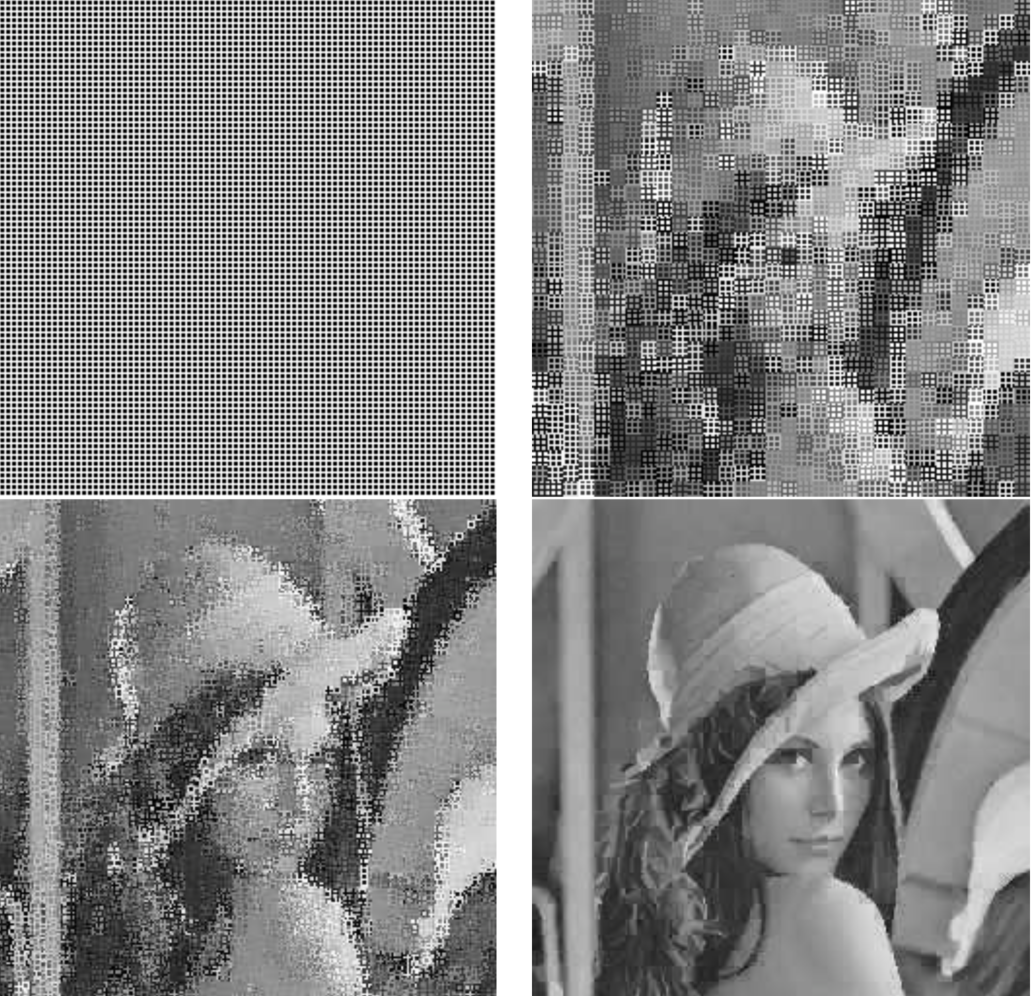
\includegraphics[width=\linewidth]{lena-pifs}
  Originalbild und decodiertes Beispielbild nach 1, 2 und 10 Iterationen.
  \marginrule{}
\end{marginfigure}

Man kann die Parameter eines PIFS beispielsweise folgendermaßen bestimmen:

\begin{enumerate}
  \item Unterteile das gegebene Bild in nicht-überlappende Quadrate (8*8 Pixel) \( R \coloneqq \left \{ R_1,\dots, R_n \right \} \).
  \item Unterteile das gegebene Bild in überlappende Quadrate (16*16 Pixel) \( D \coloneqq \left \{ D_1, \dots, D_m \right \} \).
  \item Durchsuche für jede der 8 möglichen Transformationen eines \( R_i \) alle \( D \) nach einem \( D_j \), sodass sich \( R_i \) und \( D_j \) unter der gegebenen Transformation so sehr ähneln wie möglich.
  \item Passe für jede Transformation Belichtung und Kontrast an.
\end{enumerate}

Resultat dieses Algorithmus ist ein PIFS, bestehend aus Transformationen für jedes \( R_i \in R \).



\begin{marginfigure}
  \textbf{Quellen}:
  \begin{itemize}
    \item Barnsley --- \textbf{Fractals Everywhere} (1993)
    \item Barnsley, Hurd --- \textbf{Fractal Image Compression} (1993)
    \item Fisher --- \textbf{Fractal Image Compression} (1992)
  \end{itemize}
\end{marginfigure}

\end{document}
